\documentclass[10pt,twocolumn]{article} 
\usepackage[utf8]{inputenc}
\usepackage{indentfirst}
\usepackage[english]{babel}
\usepackage[margin=1in]{geometry}
\usepackage{graphicx}
\usepackage{tikz}
\usepackage{relsize}

 
 \title{Home Automation System}
\author{Jacob Minyoung Huh, Jene Li, Michelle Nguyen}
\begin{document}
\maketitle
\section*{Introduction}
In the past, predictions of technology included visions of the future home as a fully-automated, interactive "smart home". With the rising popularity of the Internet of Things phenomenon, many attempts have been made in the field of home automation. From thermostats that can predict your desired temperature, to systems that can monitor and control the lights throughout your home, that vision of the future has been realized. However, despite such widespread pursuits in home automation, the majority of today?s modern homes do not utilize these home automation systems. Our goal is to create a home automation framework that remedies the problems of these current home automation systems. This includes creating a framework that remains connected and interactive despite losing internet connectivity. We also focus on the expandability and flexibility of our platform for easy use of both custom sensors and existing sensors already in the market. Furthermore, we design our system so that it provides a simple, intuitive interface that is easy to build any application upon, allowing us to serve as a strong platform on which to run any household's desired application. 
\section*{Overview}
For our system, we decided to focus on three core components: the sensors, the server, and the integration of the former. These are implemented over two physical modules: the sensor module and the server module. The sensor module consists of libraries that help us make our platform flexible, expandable, and easy to use. The server module employs two servers, one that is run locally, and one that is deployed on the cloud. These two modules form a concurrent system that ensures that our sensor data is always being recorded regardless of internet connectivity. The sensor data can then be accessed either locally or through the cloud via simple APIs that help simplify the application development process. The general system model of our modules can be seen in the following, where each module can further be represented as a finite state machine:
 \begin{figure}[h]
  \centering
    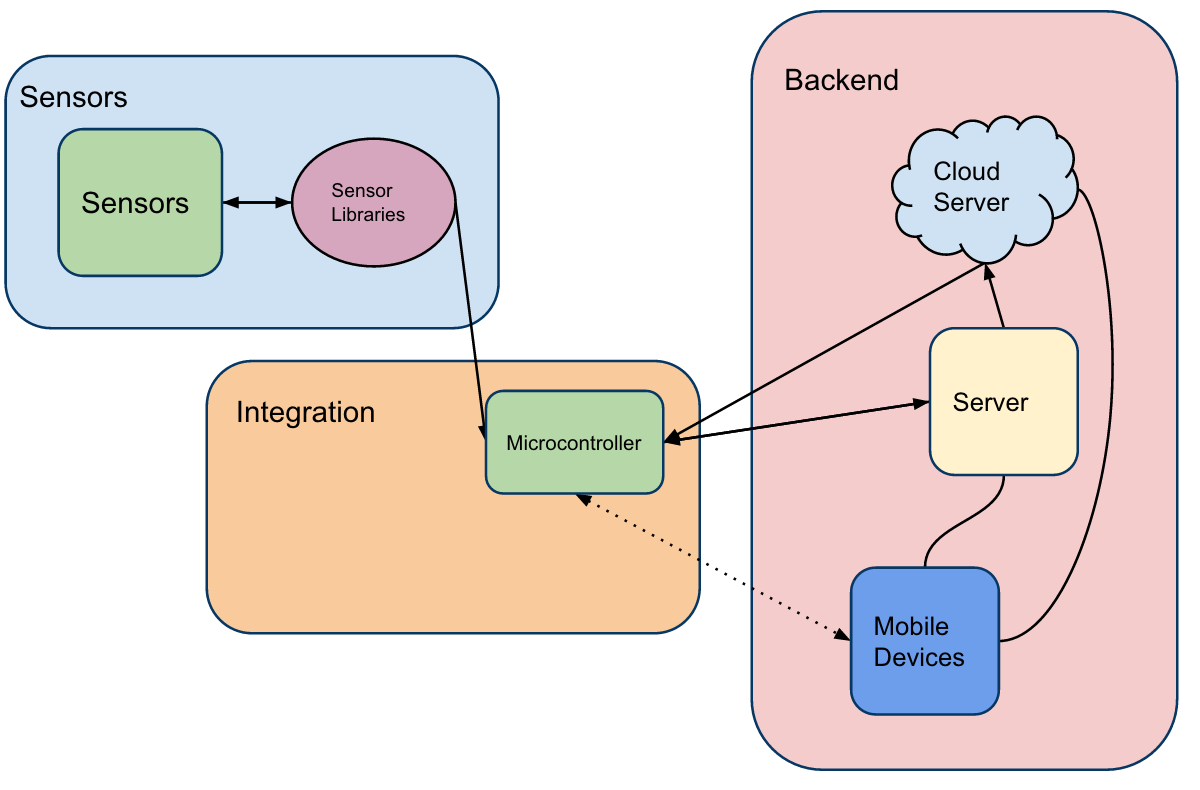
\includegraphics[scale=0.35]{generalmodel.png}
  \caption{General system model}
  \label{fig:gsm}
\end{figure}
\section*{Sensors}
The lowest level of infrastructure in the project comprises of sensors, which provide the valuable real-time data used in home automation. Manipulation and use of the real-time data are used in applications that are to be determined by the users and developers. Instead, we focus on creating solid libraries as a state machine, which allows the developers and users to employ the libraries in a reliable and effective way. By creating these libraries, we are abstracting away the details of the hardware and communication protocol so that it does not have to be handled by the backend users. 

 The sensors we have incorporated use two ways of communication. One subset of sensors uses pure analog reads, where the microcontroller reads the output pin value. The other uses the I2C protocol, in which communication between the sensor and the controllers is made through acknowledgement. I2C appealed to us because of the amount of freedom it gives to the users and the developers. Due to the fact that it does not depend on the number of pins, I2C has no limitation in the amount of sensors we can use and users are guaranteed a full range of use with just a single processor. By maximizing the capacity of a single processor, we see great potential in using these sensors for home automation.
 \subsection*{Analog Read}
 So how are the libraries actually modeled? We can view I2C libraries as an improvement upon the analog read libraries, or the analog read libraries as a subspace of the I2C libraries. The analog libraries are composed of methods which can be easily seen as a rough state flow graph. 
 \begin{figure}[h]
  \centering
    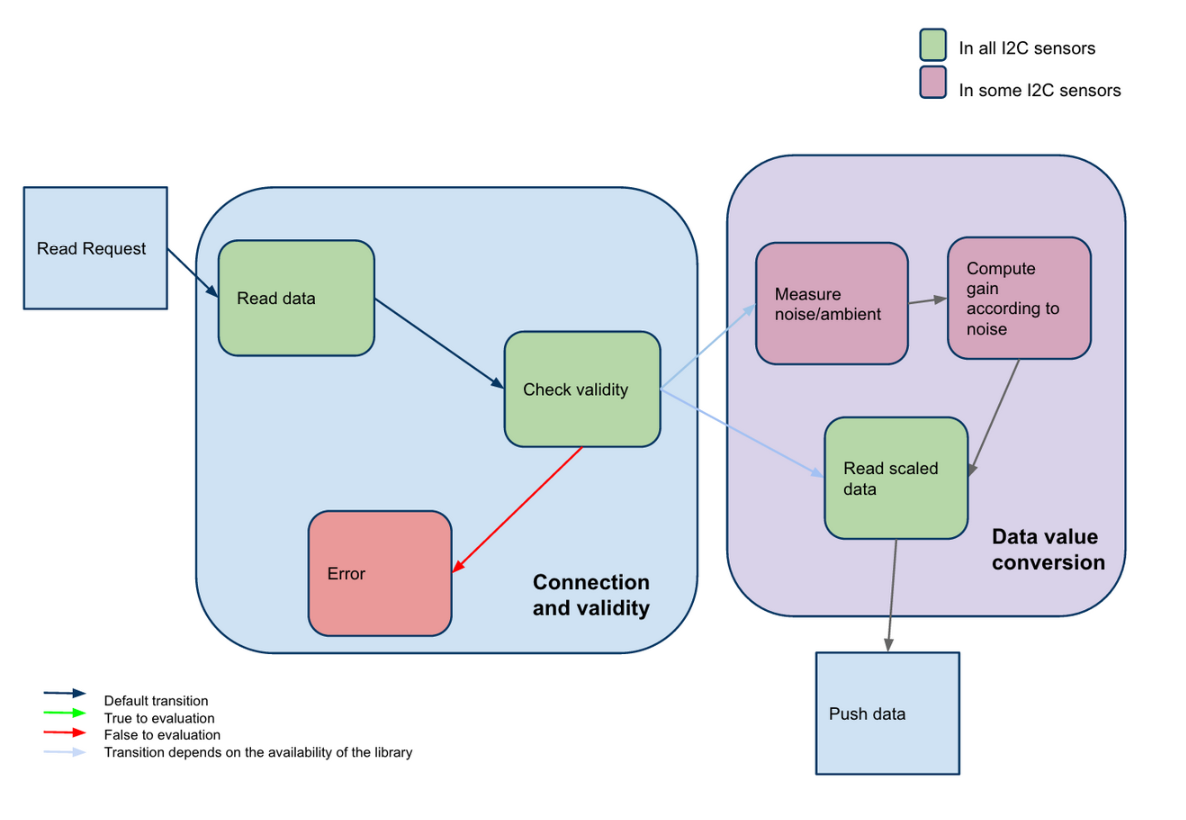
\includegraphics[scale=0.4]{analogreadsm.png}
  \caption{State flow graph for analog read libraries}
  \label{fig:analogread}
\end{figure}
Every time a reader request is made, the library calls read data and checks if it is valid. If the data read is not valid (e.g saturated or unuseful) we will acknowledge that it is not useful and notify the user that an error has occured. This step can be checked during the application. After it has ensured that it is valid, depending on the sensor, we will compute gain depending on the noise and push out the scaled, meaningful data. 
\subsection*{I2C}
Similarly to the pure analog libraries, the I2C protocols have been defined. The I2C protocol consists of acknowledgement between the master (processor) and the slave (sensors). We first check if the sensor connection has been made and additionally check if the revision number of the sensor matches the one we have seen in the data sheet. After all initialization has been done, then we can start requesting data. The unique slave address gives us the freedom to connect to multiple I2C devices.
\begin{figure}[h]
  \centering
    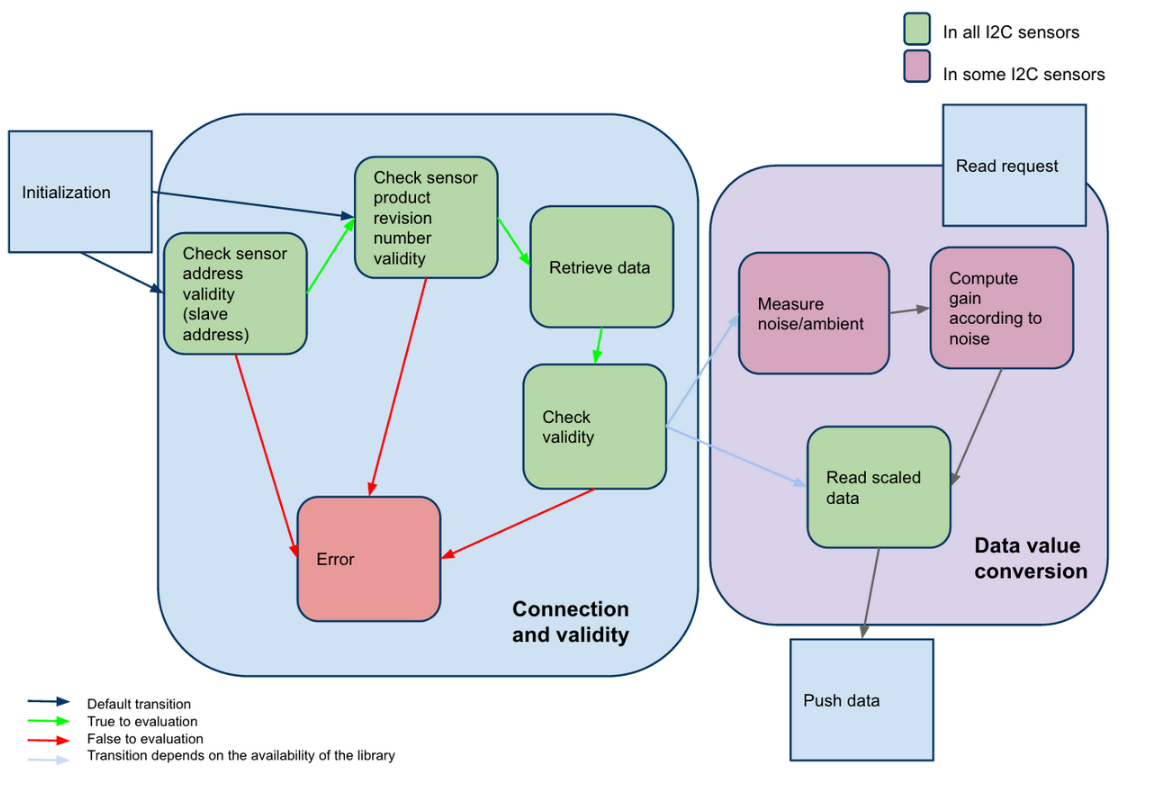
\includegraphics[scale=0.4]{ic2sm.png}
  \caption{State flow graph for IC2 libraries}
  \label{fig:ic2read}
\end{figure}

We can see that this is very similar to the pure analog read, except that we check if the initialization and connection has gone through correctly, in order to avoid reading corrupted data. Though extracting data is much more complicated than pure analog, it will not be discussed in this report. Furthermore, we can represent our I2C libraries as a state machine, which also encompasses the state machine for the analog read libraries.
\begin{figure}[h]
  \centering
    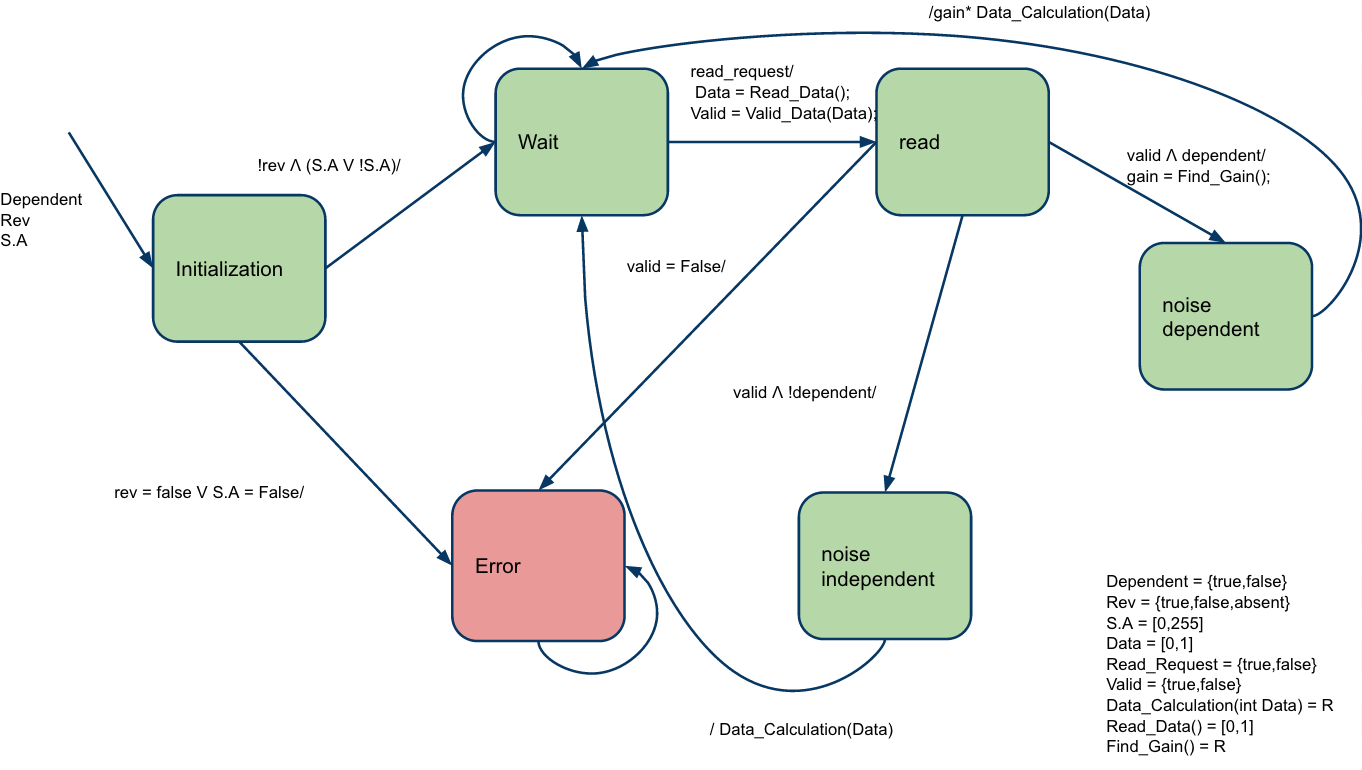
\includegraphics[scale=0.345]{libsm.png}
  \caption{State machine for IC2 and analog read libraries}
  \label{fig:sm_lib}
\end{figure}

The state machine starts with initialization. It transitions to wait if and only if initialization has finished correctly. The state machine will then stay at the wait state until an input read\_request evaluates to true. When this guard is evaluated to true, it will read data, check the validity of the read data, and transition to read. If the value that has been read is not valid for any reason, it will transition to the error state. Otherwise, it will transition according to the sensor type it is computing and push the scaled data. Finally, it will return to the wait state, where it will wait until the next request is present.

The types of sensors we have written libraries for in the project have been chosen in respect to the importance of how the real-time data impacts one's daily life. The following image includes the types of sensors and the sensor libraries we have developed.
\begin{figure}[h]
  \centering
    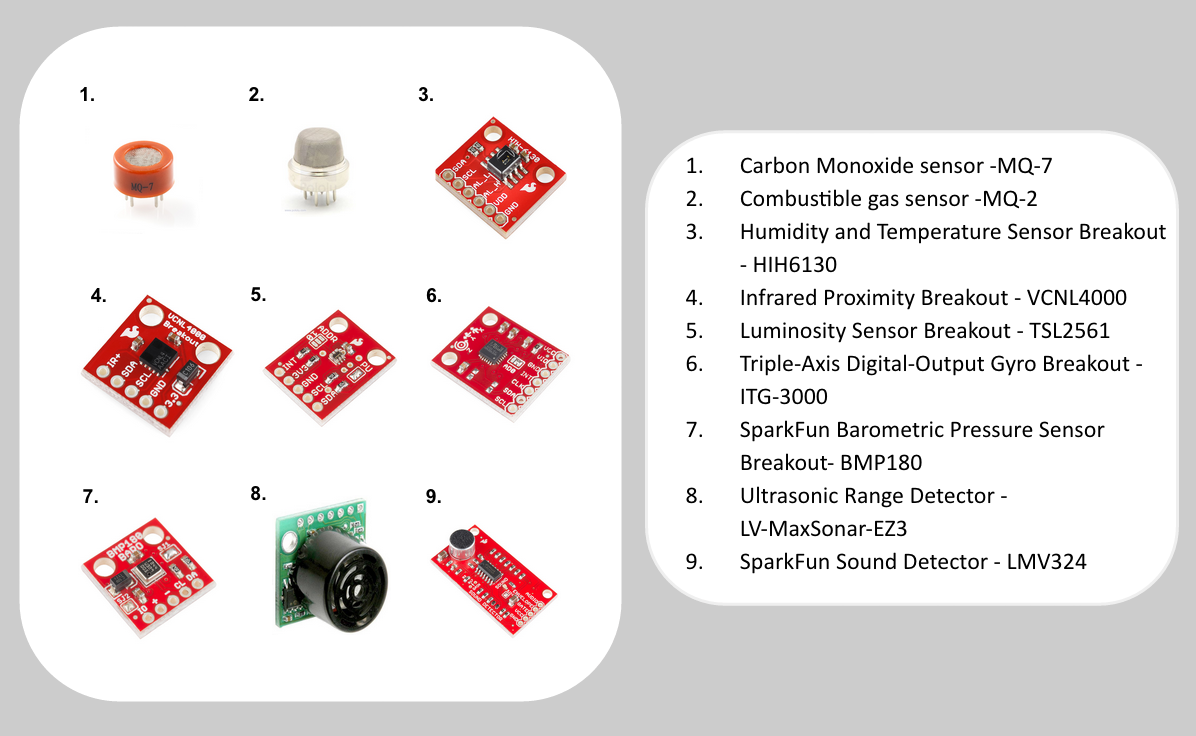
\includegraphics[scale=0.345]{sensorhardware.png}
  \caption{Sensors with written libraries}
  \label{fig:sensors}
\end{figure}
\section*{Integration}
 In order to integrate our sensor modules with our server module, we decided to use a lightweight TCP protocol over WiFi. This allows our server modules to be connected across the home wherever WiFi reaches. With the addition of a uninterrupted power source on the router, the TCP connection will always be running regardless of power loss or internet connectivity problems.
 \begin{figure}[h]
  \centering
    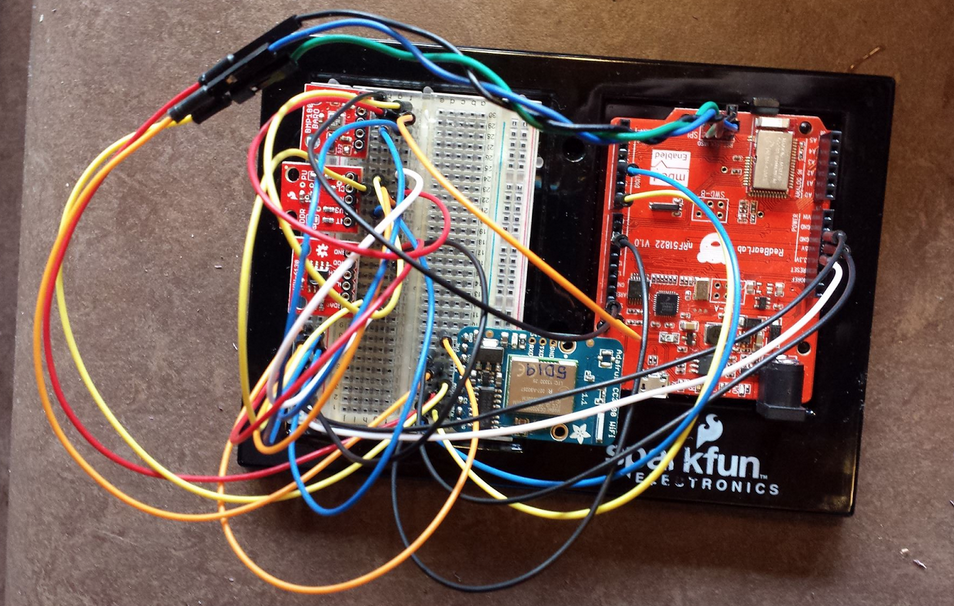
\includegraphics[scale=0.3]{integ.png}
  \caption{Demo board for integration module}
  \label{fig:integ}
\end{figure}

For our demo, we created a small application to demonstrate our system. This application uses three sensors: a humidity, barometer, and temperature sensor which constitutes as our sensor module. Using an mbed RedBearLab nRF51822 paired with an Adafruit CC3000 WiFi breakout board, our board acts as a TCP client and interfaces with the local server by sending sensor readings.\\
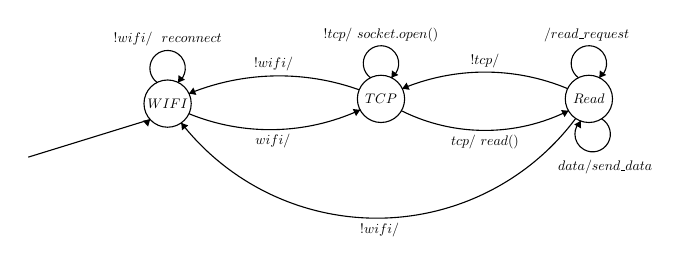
\begin{tikzpicture}[scale=0.1, every node/.style={scale=0.5}]
\tikzstyle{every node}+=[inner sep=0pt]
\draw [black] (17.7,-28.8) circle (3);
\draw (17.7,-28.8) node {$WIFI$};
\draw [black] (44.8,-28.2) circle (3);
\draw (44.8,-28.2) node {$TCP$};
\draw [black] (71.2,-28.2) circle (3);
\draw (71.2,-28.2) node {$Read$};
\draw [black] (42.15,-29.603) arc (-65.24698:-112.21635:27.285);
\fill [black] (42.15,-29.6) -- (41.21,-29.48) -- (41.63,-30.39);
\draw (31.36,-32.66) node [below] {$wifi/\mbox{ }$};
\draw [black] (68.607,-29.705) arc (-63.47645:-116.52355:23.753);
\fill [black] (68.61,-29.71) -- (67.67,-29.62) -- (68.11,-30.51);
\draw (58,-32.71) node [below] {$tcp/\mbox{ }\\read()$};
\draw [black] (69.877,-25.52) arc (234:-54:2.25);
\draw (71.2,-20.95) node [above] {$/read\_request\mbox{ }$};
\fill [black] (72.52,-25.52) -- (73.4,-25.17) -- (72.59,-24.58);
\draw [black] (43.477,-25.52) arc (234:-54:2.25);
\draw (44.8,-20.95) node [above] {$!tcp/\mbox{ }\\socket.open()$};
\fill [black] (46.12,-25.52) -- (47,-25.17) -- (46.19,-24.58);
\draw [black] (16.377,-26.12) arc (234:-54:2.25);
\draw (17.7,-21.55) node [above] {$!wifi/\mbox{ }\\\mbox{ }reconnect$};
\fill [black] (19.02,-26.12) -- (19.9,-25.77) -- (19.09,-25.18);
\draw [black] (20.415,-27.527) arc (112.26464:70.27203:30.171);
\fill [black] (20.42,-27.53) -- (21.35,-27.69) -- (20.97,-26.76);
\draw (31.15,-24.73) node [above] {$!wifi/$};
\draw [black] (47.5,-26.896) arc (112.62805:67.37195:27.29);
\fill [black] (47.5,-26.9) -- (48.43,-27.05) -- (48.05,-26.13);
\draw (58,-24.3) node [above] {$!tcp/$};
\draw [black] (0,-35.6) -- (15.48,-30.82);
\fill [black] (15.48,-30.82) -- (14.55,-30.98) -- (15.22,-31.72);
\draw [black] (69.522,-30.686) arc (-36.74281:-141.9721:31.522);
\fill [black] (19.43,-31.25) -- (19.53,-32.19) -- (20.32,-31.57);
\draw (44.62,-43.88) node [below] {$!wifi/$};
\draw [black] (72.798,-30.725) arc (60.06798:-227.93202:2.25);
\draw (73.27,-35.95) node [below] {$data/send\_data$};
\fill [black] (70.17,-31) -- (69.34,-31.45) -- (70.2,-31.95);
\end{tikzpicture}
Our demo application can be modeled by the above chart in addition to the sensor FSM running concurrently. When in the READ state, the FSM outputs a read\_request signal that is fed into the application FSM. When data is received, it then sends it over to the server over the TCP connection. If the server connection is disconnected, it will halt reading and attempt to reconnect. This leads to the following feedback model of our concurrent system.

\begin{figure}[h]
  \centering
    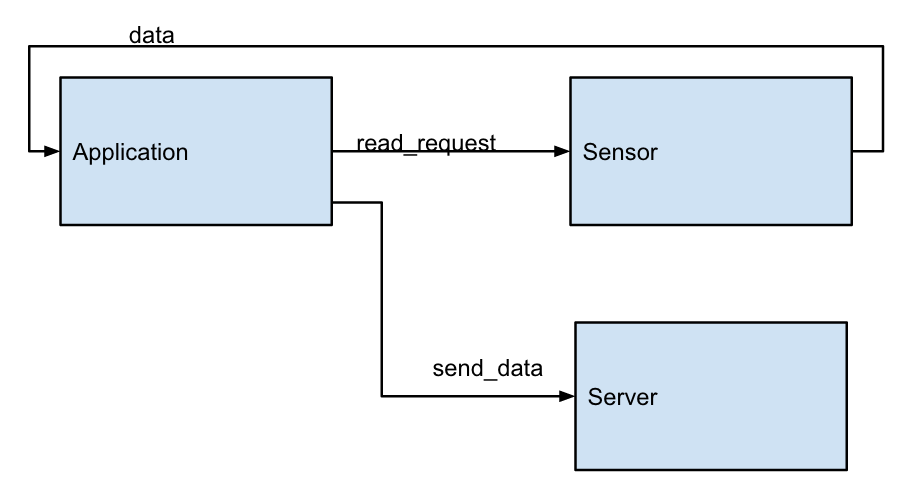
\includegraphics[scale=0.35]{feedback.png}
  \caption{Integration concurrent model}
  \label{fig:integ}
\end{figure}
\section*{Backend}
The backend consists of two servers--one that is run locally on a mbed board, and another which is deployed to the cloud. Both servers aggregate and store the collected sensor data, which the user can access through simple, intuitive interfaces.  
\subsection*{Local Server}
\begin{figure}[h]
  \centering
    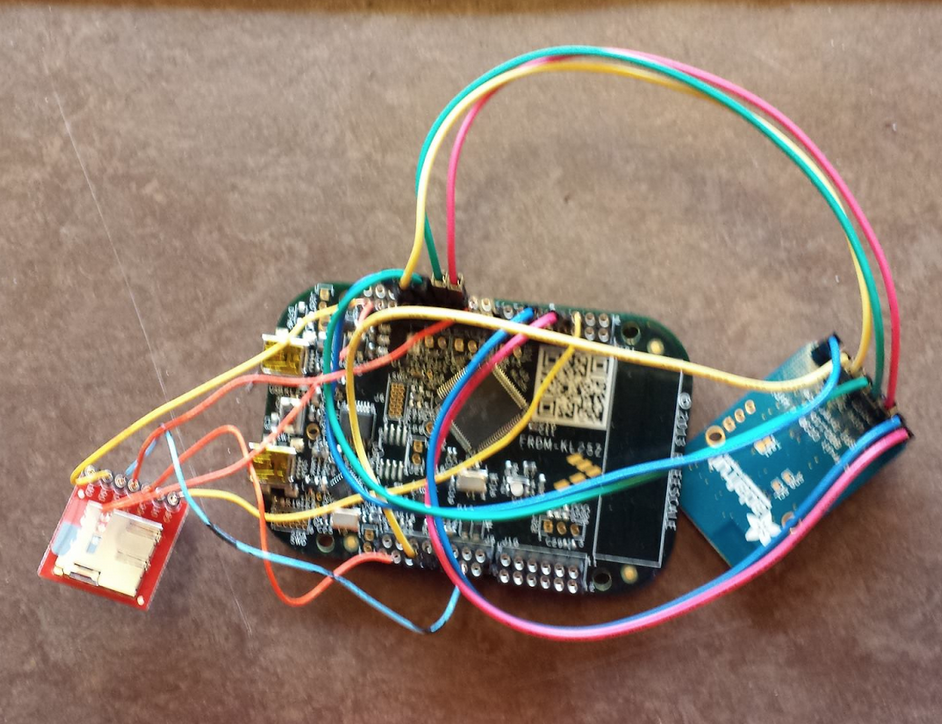
\includegraphics[scale=0.3]{server.png}
  \caption{mbed board for the local server}
  \label{fig:local_server}
\end{figure}
The local server is running on a mbed FRDM-KL25Z with an Adafruit CC3000 WiFi breakout board for internet connectivity. It is also connected to a SparkFun MicroSD breakout board so that the sensor data can safely be stored, mitigating the loss of data during any possible power outages. The local server acts as a TCP server, which polls and waits for requests from clients. These requests may add new sensor data to the server, or may get existing sensor data from the server. This is done using simple payload formats that bear a slight resemblance to those of a RESTful API, allowing it to be intuitive to use. To send data to the server, the payload format is "POST sensorname value", which will save the value for the sensor with that sensor name, and return the id of the entry that has just been stored. Similarly, if a user wants to access data on the local server, the payload format is "GET sensorname id", where the id of the entry they want is the same as the one given when the data is POSTed. The server is flexible and allows for any sensor name, and thus any type or number of sensors, to be stored. 

When connected to the internet, the local server also relays data to the cloud server as it receives the data. However, during periods of no internet access, the server notes which data entries have not yet been pushed to the cloud. A timed interrupt which is scheduled for every five minutes, checks whether there is internet connectivity, and if so, will push these updates to the cloud. Similarly, another timed interrupt scheduled for every ten minutes will attempt to reconnect the server to the internet if there is currently no internet access. We see that our home automation system differs from several other platforms which take a "Cloud-First" approach, which renders the platform unusable during network outages.
\begin{figure}[h]
  \centering
    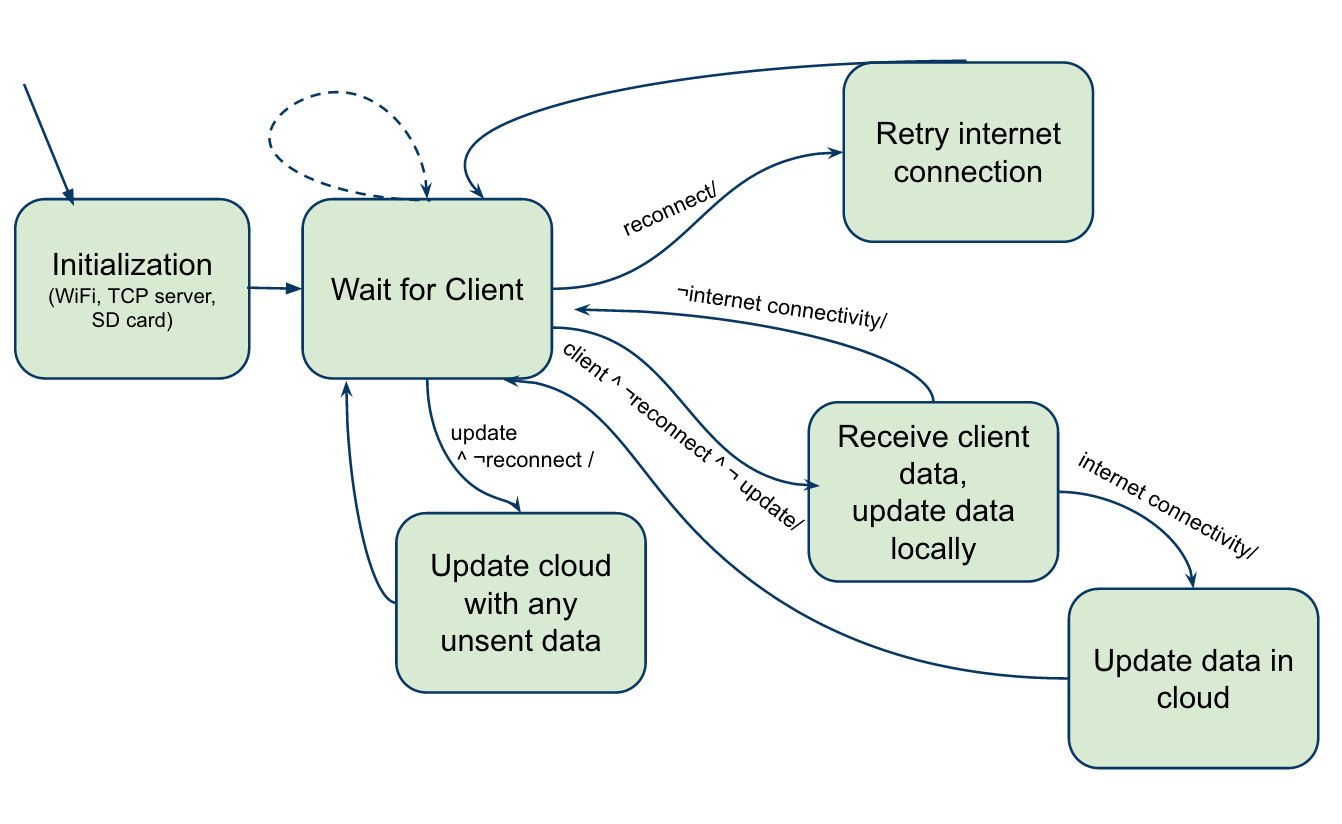
\includegraphics[scale=0.35]{localserversm.png}
  \caption{State machine for the local server}
  \label{fig:local_server_sm}
\end{figure}

The state chart for the local server is above. We see that after initializing, the server begins to wait for clients. From here, it can either receive a client, or execute an attempt to reconnect to the internet or send updates to the cloud server. After each action, it will return to its polling state.
\subsection*{Cloud Server}
The cloud server is deployed via Heroku, at ee149has.herokuapp.com, and uses a web.py framework for the Python server. This server aggregates all of the data sent by the local server and safely stores that information in the cloud. This allows users to access all of the available information and monitor their home regardless of where they are. Accessing or sending data is done through a RESTful API. This familiar protocol style allows users to easily query for the data they need, making it simple to build applications upon our architecture. Users can either choose to receive a single sensor value by providing an id, or, if no id is provided, they can receive all of the sensor data via a JSON format. 

\section*{Conclusion}
We have created an architecture that is easily usable and extendable through the design of core sensor libraries. By integrating our sensor module with our local server module, we are able to provide a working service regardless of internet connectivity. We then further improve the robustness of our system by utilizing a cloud server, also allowing users and their applications access to data beyond the home. Furthermore, we offer simple, intuitive APIs that users can easily employ to build applications without any limits. 
\subsection*{Future Work}
Now that we have an architecturally robust attempt at a home automation system, our next step would be to create a rugged enclosure for our modules so that they will be physically robust and easier on the eyes. Since our boards also support Bluetooth Low Energy, we would like to look into an identity detection feature by scanning the Bluetooth IDs of passing phones. This will add another element to our system that goes beyond what sensors can capture. It will allow us to provide users with the ability to monitor people in their home, such as who has entered a room at what time. We also want to improve our local backend server so that it attempts to reconnect to the internet in a smarter fashion. Instead of using a timed interrupt, attempting to reconnect when first detecting the WiFi has disconnected, then increasing the time between each attempt with exponential backoff, would increase the time that the local server is connected to the internet while also reducing the number of wasteful attempts.


\end{document}